\documentclass[12pt,a4paper]{report}
\usepackage[T2A]{fontenc}
\usepackage[utf8]{inputenc}
\usepackage[russian]{babel}
\usepackage{graphicx, setspace}
\usepackage{amsmath}

\usepackage[
top = 1.25cm, 
bottom = 2.0cm]{geometry}

\begin{document}
\begin{titlepage} 
	\centering
    % HEADER
	{
        \scshape
        Федеральное государственное автономное образовательное учреждение высшего образования
        \par
        \textbf{«Научно-образовательная корпорация ИТМО»}
        \par
        \vspace*{1cm}
        Факультет Программной Инженерии и Компьютерной Техники
        \par
    }
    % LOGO
    \vspace*{0.6cm}
    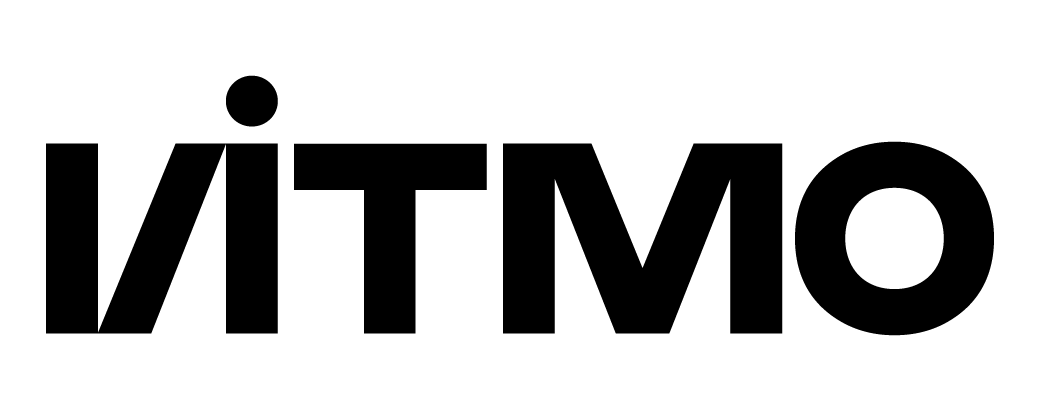
\includegraphics[width=\textwidth]{logo.png}
    % LAB INFO
    {
        \Large
        \textbf{Домашняя работа №1 по предмету\\<<Компьютерные сети>>}
        \par
        \normalsize
        \vspace*{0.75cm}
        \textbf{Вариант САА}
        \par
    }
    \vfill
    % СREDITS
    \hfill\begin{minipage}{\dimexpr\textwidth-7.8cm}
        \textbf{Выполнил:}\par
        Степанов Арсений Алексеевич\par
        \vspace*{0.15cm}
        \textbf{Группа:}\par
        P3318\par
        \vspace*{0.15cm}
        \textbf{Преподаватель:}\par
        Тропченко Андрей Александрович\par
    \end{minipage}
    \vfill
    Санкт-Петербург, \the\year{}г.
\end{titlepage}  
\section*{Задание}
Изучение методов физического и логического кодирования. Необходимо:
\begin{enumerate}
    \item Сформировать исходное сообщение
    \item Закодировать одно и то же бинарное сообщение несколькими методами, Manchester обязательно и минимум 3 варианта на выбор
    \begin{itemize}
        \item Manchester
        \item NRZ
        \item RZ
        \item AMI
        \item MLT-3
        \item NRZI
        \item PAM-5
        \item Differential Manchester
    \end{itemize}
    \item Для каждого метода необходимо
    \begin{itemize}
        \item Нарисовать временную диаграмму сигнала
        \item Рассчитать частоты (при скорости канала 100 Мбит/с):
        \begin{itemize}
            \item верхнюю частоту
            \item нижнюю частоту
            \item спектр сигнала
            \item среднюю частоту
            \item требуемую полосу пропускания
        \end{itemize}
        \item Сделать таблицу сравнения методов
        \item Выписать плюсы и минусы
    \end{itemize}
    \item Выбрать один из методов физического кодирования из предыдущего этапа и:
    \begin{itemize}
        \item Применить кодирование 4B/5B
        \item Записать результат
        \begin{itemize}
            \item в binary
            \item в hex
        \end{itemize}
        \item Определить
        \begin{itemize}
            \item новую длину сообщения
            \item избыточность
        \end{itemize}
        \item Нарисовать временную диаграмму
        \item Снова посчитать:
        \begin{itemize}
            \item верхнюю частоту
            \item нижнюю частоту
            \item среднюю частоту
            \item полосу пропускания
        \end{itemize}
        \item Сравнить с физическим кодированием
    \end{itemize}
    \item Скремблирование
    \begin{itemize}
        \item Нужно применить scrambler, выбрать один полином:
        \begin{itemize}
            \item $B_i = A_i \oplus B_{i-3} \oplus B_{i-5}$
            \item $B_i = A_i \oplus B_{i-5} \oplus B_{i-7}$
        \end{itemize}
        \item Вычислить скремблированную последовательность
        \item Записать
        \begin{itemize}
            \item binary
            \item hex
        \end{itemize}
        \item Нарисовать временную диаграмму
        \item Снова вычислить
        \begin{itemize}
            \item верхнюю частоту
            \item нижнюю частоту
            \item среднюю
            \item полосу пропускания
        \end{itemize}
    \end{itemize}
    \item Сделать итоговый сравнительный анализ
    \begin{itemize}
        \item Сформировать таблицу
        \begin{itemize}
            \item Метод
            \item $F_\text{н}$
            \item $F_\text{в}$
            \item средняя
            \item спектр
            \item полоса
        \end{itemize}
        \item Включить в таблицу
        \begin{itemize}
            \item методы из этапа 2
            \item метод 4B/5B
            \item метод со скремблером
        \end{itemize}
        \item Написать вывод
        \item Выбрать лучший метод кодирования
    \end{itemize}
\end{enumerate}
\newpage
\section*{Выполнение}
\subsection*{Формирование сообщения}
\begin{itemize}
    \item Исходное сообщение: \textbf{САА}
    \item Представление в hex: \textbf{D1 C0 C0}
    \item Преставление в bin: \textbf{1101 0001 1100 0000 1100 0000}
    \item Длина сообщения: \textbf{3 байта (24 бит)}
\end{itemize}
\subsection*{Физическое кодирование исходного сообщения}
\subsubsection*{Манчестерское кодирование}
\begin{itemize}
    \item Верхняя граница частот: $F_\text{в}=C=100 \text{МГц}$
    \item Нижняя граница частот: $F_\text{н}=\dfrac{C}{2}= 50 \text{МГц}$
    \item Середина спектра: $F_{\frac{1}{2}}=\dfrac{F_\text{в} + F_\text{н}}{2}=75 \text{МГц}$
    \item Ширина спектра: $S = F_\text{в} - F_\text{н} = 50\text{МГц}$
\end{itemize}
\begin{center}
    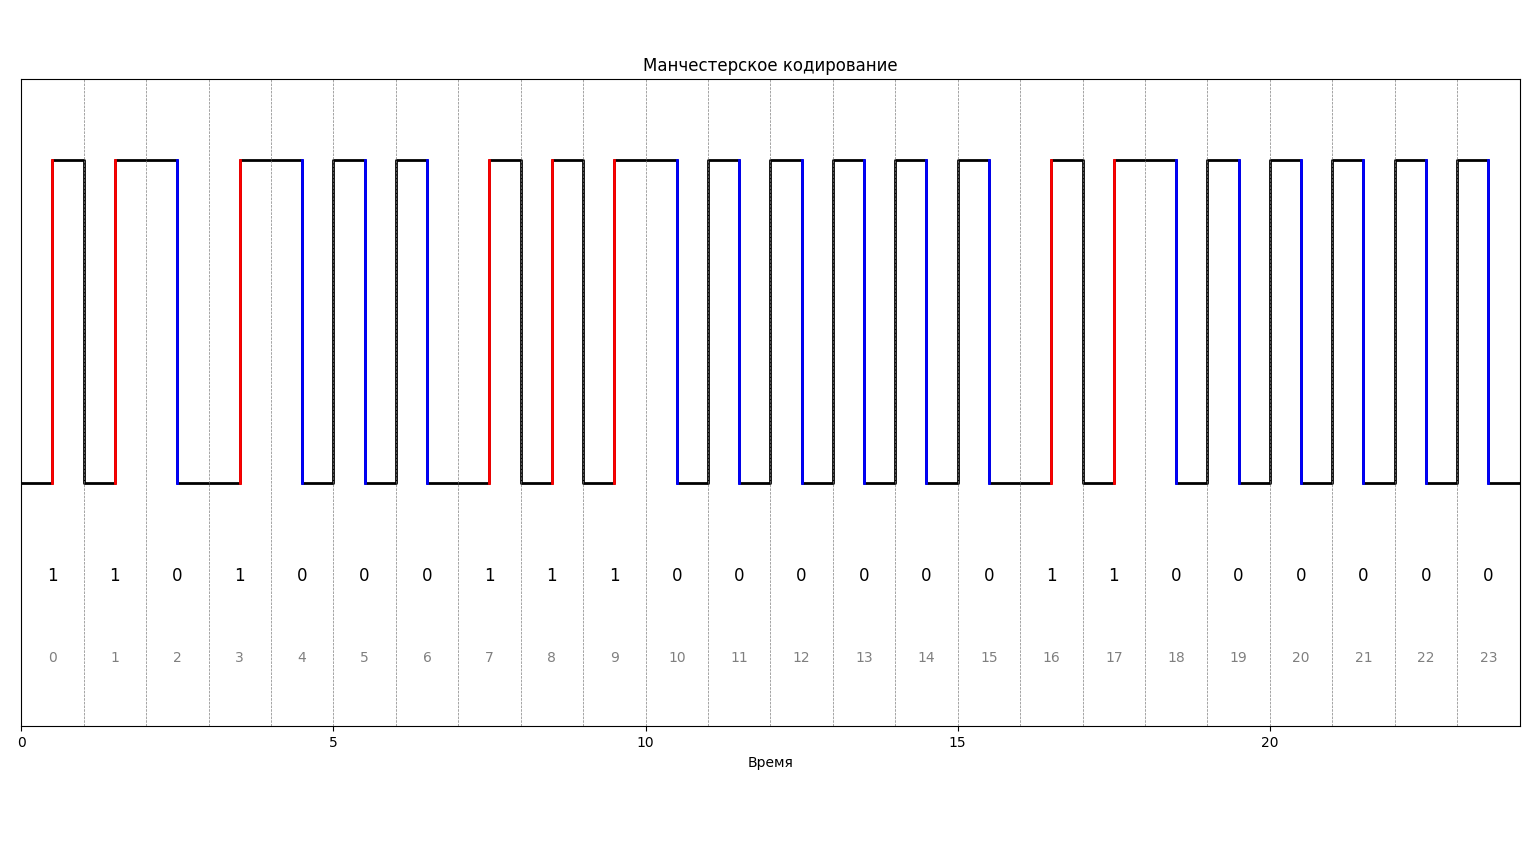
\includegraphics[width=\textwidth]{assets/manchester.png}
\end{center}
\subsubsection*{Кодирование методом NRZ}
Анализ последовательности:
\begin{center}
    \textbf{11 | 0 | 1 | 000 | 111 | 000000 | 11 | 000000}
\end{center}
\begin{center}
    \begin{tabular}{cc}
        Длина & Кол-во серий \\
        1 & 2 \\
        2 & 2 \\
        3 & 2 \\
        6 & 2
    \end{tabular}
\end{center}
$$n_\text{max} = 6$$


\begin{itemize}
    \item Верхняя граница частот: $F_\text{в}=\dfrac{C}{2}=50 \text{МГц}$
    \item Нижняя граница частот: $F_\text{н}=\dfrac{C}{2 \cdot n_\text{max}}=\dfrac{C}{12}= 8.333 \text{МГц}$
    \item Середина спектра: $F_{\frac{1}{2}}=\dfrac{F_\text{в} + F_\text{н}}{2}=29.166 \text{МГц}$
    \item Средняя частота спектра: $F_\text{ср}=\dfrac{2\cdot\frac{F_\text{в}}{1} + 4\cdot\frac{F_\text{в}}{2}+ 6\cdot\frac{F_\text{в}}{3} + 12\cdot\frac{F_\text{в}}{6}}{24}=16.667\text{МГц}$
    \item Ширина спектра: $S = F_\text{в} - F_\text{н} = 41.667\text{МГц}$
    \item Полоса пропускания: $F=\dfrac{C}{2}=50\text{МГц}$
\end{itemize}
\begin{center}
    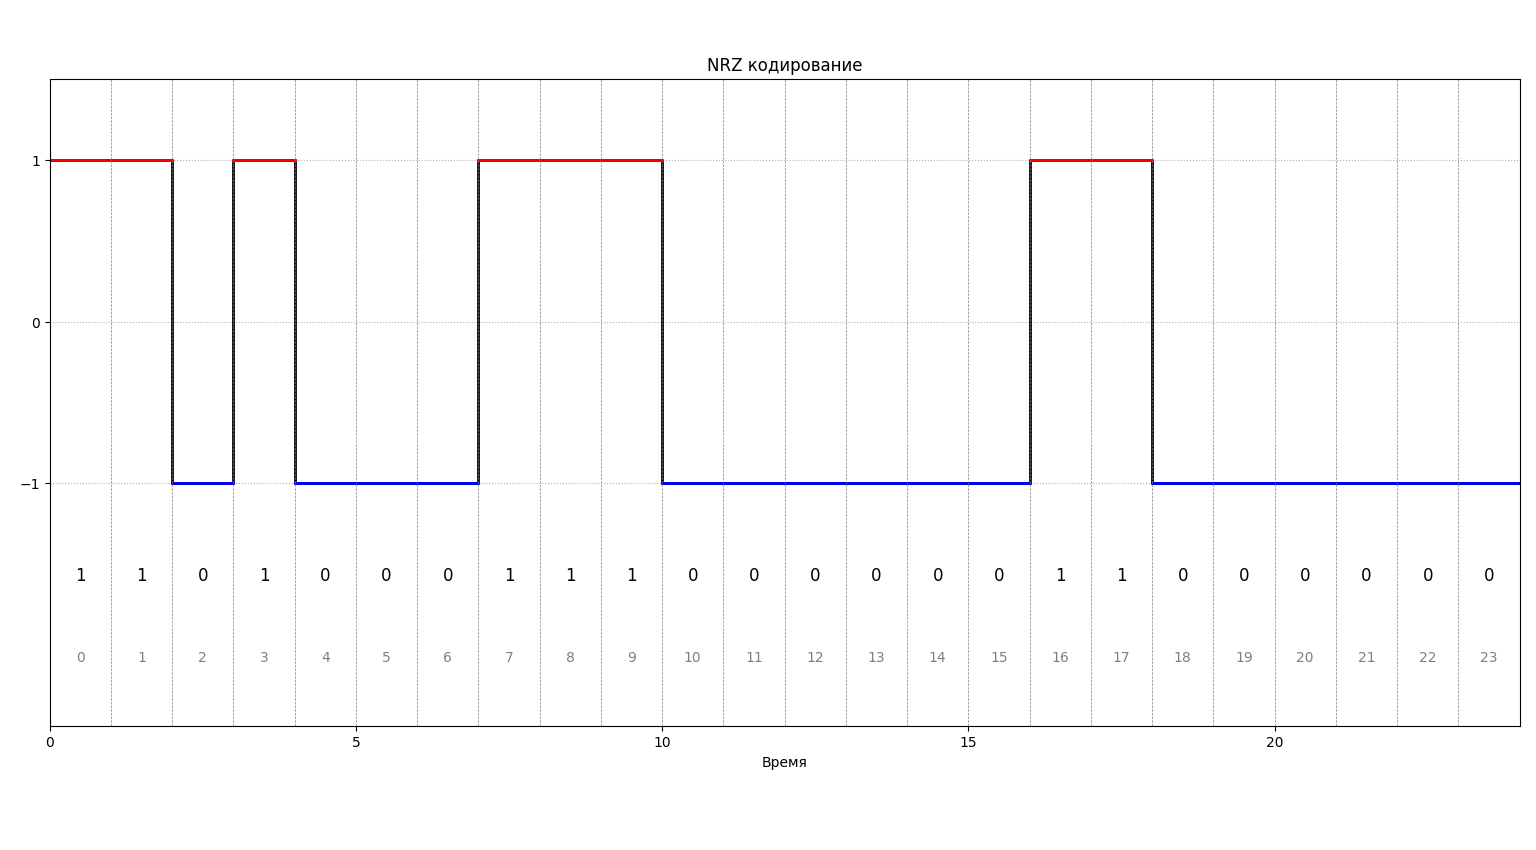
\includegraphics[width=\textwidth]{assets/nrz.png}
\end{center}
\subsubsection*{Кодирование методом RZ}
\begin{itemize}
    \item Верхняя граница частот: $F_\text{в}=C=100 \text{МГц}$
    \item Нижняя граница частот: $F_\text{н}=\dfrac{C}{2}= 50 \text{МГц}$
    \item Середина спектра: $F_{\frac{1}{2}}=\dfrac{F_\text{в} + F_\text{н}}{2}=75 \text{МГц}$
    \item Средняя частота спектра: $F_\text{ср}=\dfrac{24\cdot F_\text{в} + 8 \cdot F_\text{н}}{24}=87.5\text{МГц}$
    \item Ширина спектра: $S = F_\text{в} - F_\text{н} = 50\text{МГц}$
    \item Полоса пропускания: $F=\dfrac{C}{2}=50\text{МГц}$
\end{itemize}
\begin{center}
    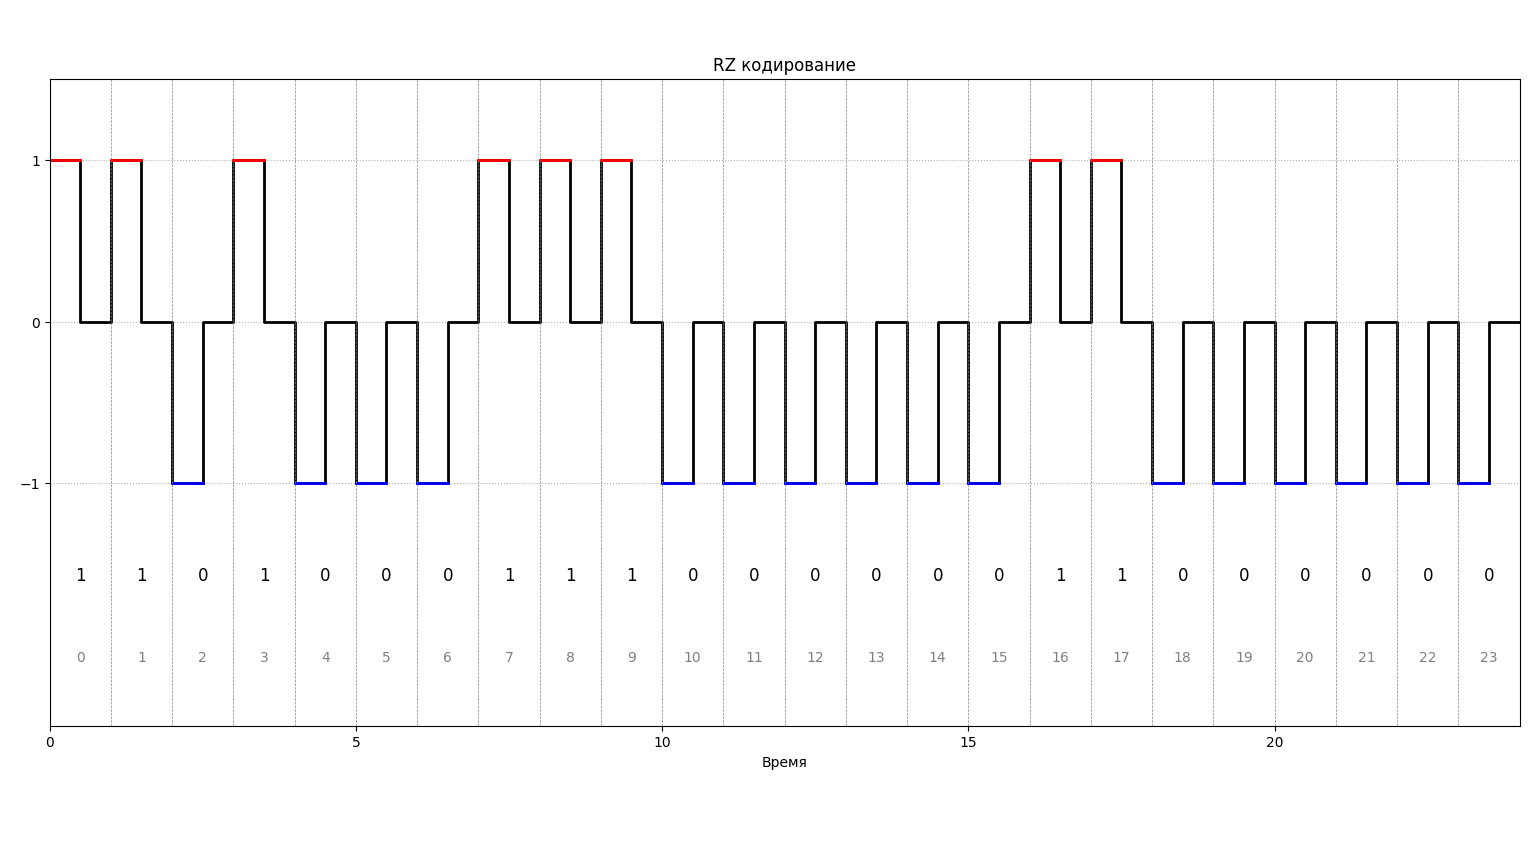
\includegraphics[width=\textwidth]{assets/rz.png}
\end{center}
\subsubsection*{Кодирование методом AMI}
\begin{itemize}
    \item Верхняя граница частот: $F_\text{в}=\dfrac{C}{2}=50 \text{МГц}$
    \item Нижняя граница частот: $F_\text{н}=\dfrac{C}{2\cdot(n_{\text{max}} + 1)} = 7.143 \text{МГц}$
    \item Середина спектра: $F_{\frac{1}{2}}=\dfrac{F_\text{в} + F_\text{н}}{2}=28.571 \text{МГц}$
    \item Средняя частота спектра: $F_\text{ср}=\dfrac{8}{24}\cdot\dfrac{C}{2}=16.667\text{МГц}$
    \item Ширина спектра: $S = F_\text{в} - F_\text{н} = 42.857\text{МГц}$
    \item Полоса пропускания: $F=\dfrac{C}{2}=50\text{МГц}$
\end{itemize}
\begin{center}
    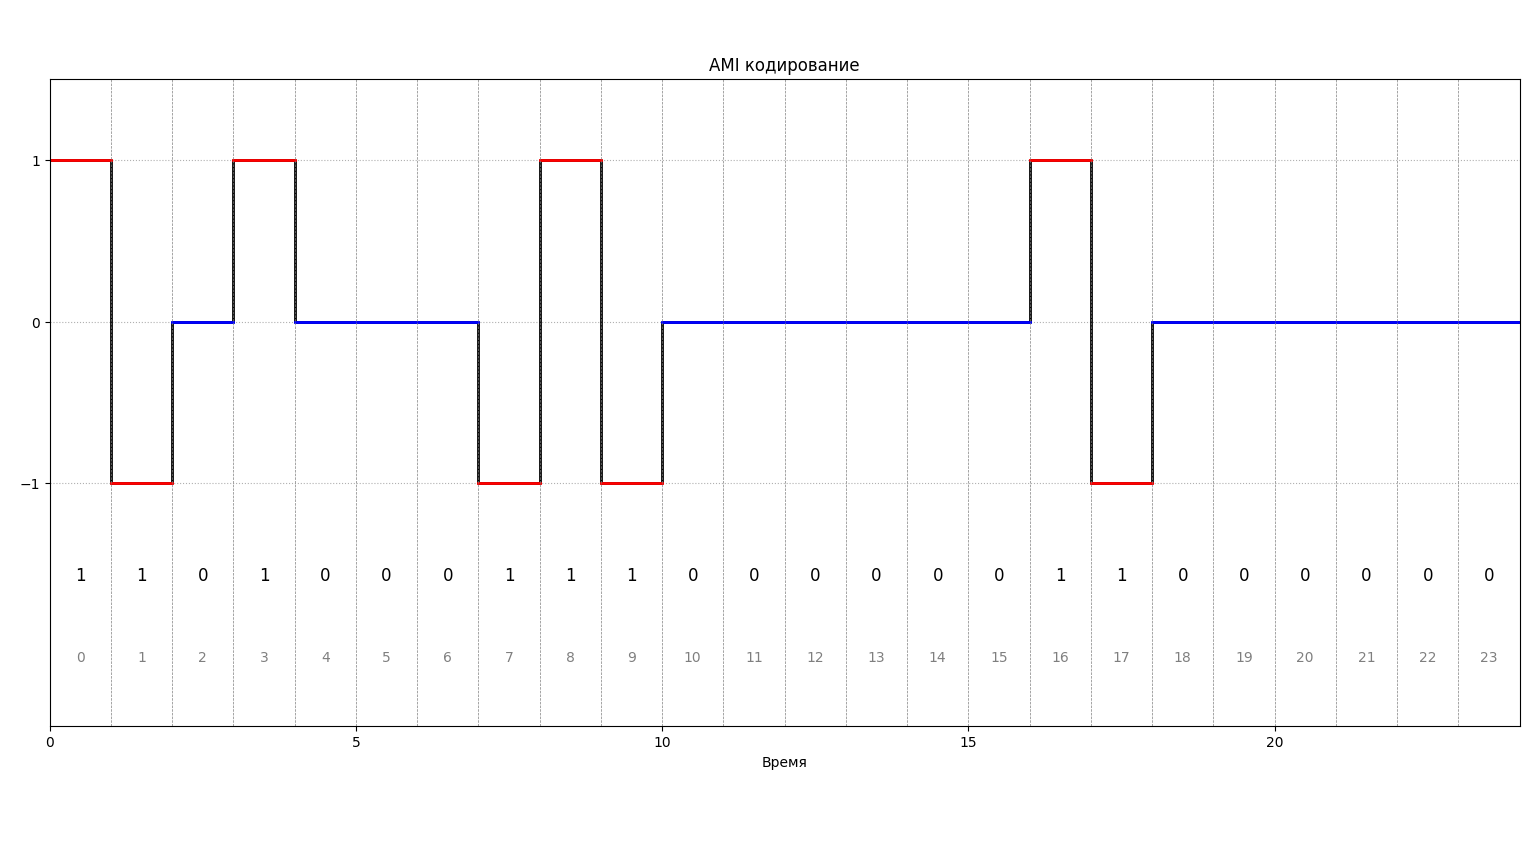
\includegraphics[width=\textwidth]{assets/ami.png}
\end{center}
\subsubsection*{Сравнительный анализ}
\begin{tabular}{|l|c|c|c|c|}
    \hline
    \textbf{Метод кодирования} & Манчестерская & NRZ & RZ & AMI \\
    \hline
    \textbf{Полоса пропускания} & 100МГц & 50МГц & 100МГц & 50МГц \\
    \hline
    \textbf{Самосинхронизация} & Есть & Нет & Есть & Нет \\
    \hline
    \textbf{Постоянная составляющая} & Нет & Есть & Нет & Есть \\
    \hline
    \textbf{Уровни сигнала} & 2 & 2 & 3 & 3 \\
    \hline
    \textbf{Эффективность} & Низкая & Высокая & Низкая & Высокая \\
    \hline
\end{tabular}
\hfill\break
\textbf{Манчестерское кодирование}
\begin{itemize}
    \item Плюсы
    \begin{itemize}
        \item Самосинхронизация, даже при длинных последовательностях
        \item Отсутствует постоянная составляющая
        \item Лёгкое обнаружение ошибок
    \end{itemize}
    \item Минусы
    \begin{itemize}
        \item Требует большей полосы пропускания
        \item Меньшая скорость
    \end{itemize}
\end{itemize}
\textbf{NRZ кодирование}
\begin{itemize}
    \item Плюсы
    \begin{itemize}
        \item Простота реализации
        \item Эффективность использования полосы
    \end{itemize}
    \item Минусы
    \begin{itemize}
        \item Проблема с синхронизацией
        \item Нет механизмов обнаружения ошибок
    \end{itemize}
\end{itemize}
\textbf{RZ кодирование}
\begin{itemize}
    \item Плюсы
    \begin{itemize}
        \item Синхронизация лучше чем в NRZ
    \end{itemize}
    \item Минусы
    \begin{itemize}
        \item Сложность реализации
        \item Требует в 2 раза больше полосы относительно NRZ
        \item Малая эффективность
    \end{itemize}
\end{itemize}
\textbf{AMI кодирование}
\begin{itemize}
    \item Плюсы
    \begin{itemize}
        \item Отсутствует постоянная составляющая
        \item Обнаружение ошибок
        \item Эффективность
    \end{itemize}
    \item Минусы
    \begin{itemize}
        \item Потеря синхронизации при длительной последовательности нулей
        \item Необходимость в скремблировании
    \end{itemize}
\end{itemize}

\subsection*{Логическое кодирование исходного сообщения}
\begin{itemize}
    \item Исходное сообщение: \textbf{1101 0001 1100 0000 1100 0000}
    \item Закодированое сообщение: \textbf{11011 01001 11010 11110 11010 11110}
    \item Представление закодированного сообщения в hex: \textbf{36 9D 7B 5E}
    \item Длина сообщения: \textbf{3.75 байта (30 бит)}
    \item Избыточность: \textbf{25\%}
\end{itemize}
Анализ новой последовательности:
\begin{center}
    \textbf{11 | 0 | 11 | 0 | 1 | 00 | 111 | 0 | 1 | 0 | 1111 | 0 | 11 | 0 | 1 | 0 | 1111 | 0}
\end{center}
\begin{center}
    \begin{tabular}{cc}
        Длина & Кол-во серий \\
        1 & 11 \\
        2 & 4 \\
        3 & 1 \\
        4 & 2
    \end{tabular}
\end{center}
$$n_\text{max} = 4$$
\begin{itemize}
    \item Верхняя граница частот: $F_\text{в}=\dfrac{C}{2}=50 \text{МГц}$
    \item Нижняя граница частот: $F_\text{н}=\dfrac{C}{2 \cdot n_\text{max}}=\dfrac{C}{8}= 12.5 \text{МГц}$
    \item Середина спектра: $F_{\frac{1}{2}}=\dfrac{F_\text{в} + F_\text{н}}{2}=31.25 \text{МГц}$
    \item Средняя частота спектра: $F_\text{ср}=\dfrac{11\cdot\frac{F_\text{в}}{1} + 4\cdot\frac{F_\text{в}}{2}+ 1\cdot\frac{F_\text{в}}{3} + 2\cdot\frac{F_\text{в}}{4}}{24}=28.819\text{МГц}$
    \item Ширина спектра: $S = F_\text{в} - F_\text{н} = 38\text{МГц}$
    \item Полоса пропускания: $F=\dfrac{C}{2}=50\text{МГц}$
\end{itemize}
\begin{center}
    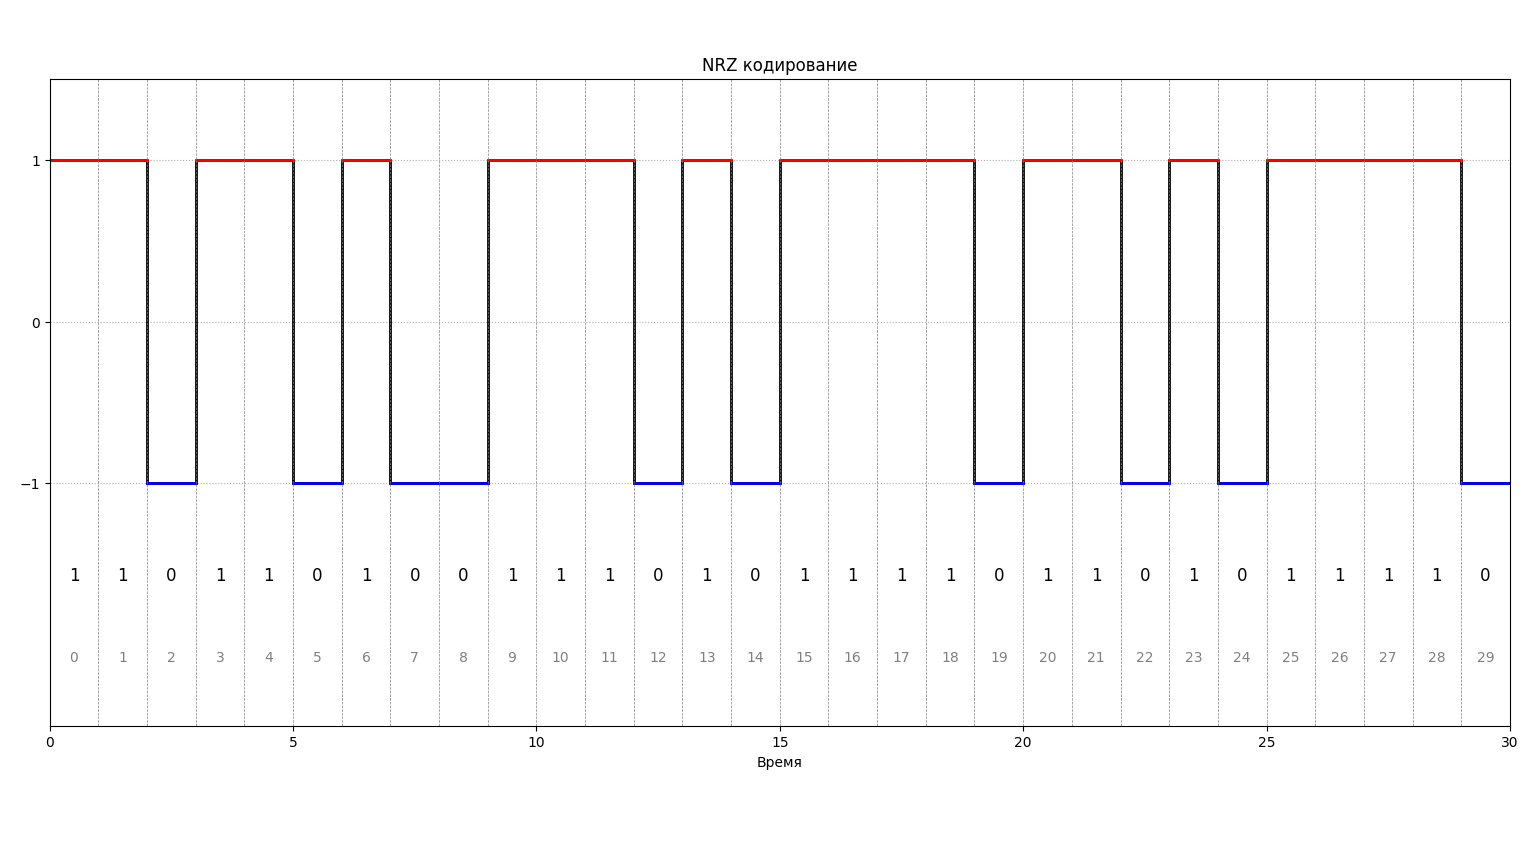
\includegraphics[width=\textwidth]{assets/nrz-4b-5b.png}
\end{center}

\subsection*{Скремблирование}
Для скремблирования выберем полином $B_i = A_i \oplus B_{i-5} \oplus B_{i-7}$

$$
\begin{array}{lllllll}
    A_{1} = 1 & & B_1 & = & A_1 & = & 1 \\
    A_{2} = 1 & & B_2 & = & A_2 & = & 1 \\
    A_{3} = 0 & & B_3 & = & A_3 & = & 0 \\
    A_{4} = 1 & & B_4 & = & A_4 & = & 1 \\
    A_{5} = 0 & & B_5 & = & A_5 & = & 0 \\
    A_{6} = 0 & & B_6 & = & A_6 & = & 1 \\
    A_{7} = 0 & & B_{7} & = & A_{7} \oplus B_{2} & = & 1 \\
    A_{8} = 1 & & B_{8} & = & A_{8} \oplus B_{3} & = & 0 \\
    A_{9} = 1 & & B_{9} & = & A_{9} \oplus B_{4} \oplus B_{2} & = & 1 \\
    A_{10} = 1 & & B_{10} & = & A_{10} \oplus B_{5} \oplus B_{3} & = & 1 \\
    A_{11} = 0 & & B_{11} & = & A_{11} \oplus B_{6} \oplus B_{4} & = & 0 \\
    A_{12} = 0 & & B_{12} & = & A_{12} \oplus B_{7} \oplus B_{5} & = & 1 \\
    A_{13} = 0 & & B_{13} & = & A_{13} \oplus B_{8} \oplus B_{6} & = & 1 \\
    A_{14} = 0 & & B_{14} & = & A_{14} \oplus B_{9} \oplus B_{7} & = & 0 \\
    A_{15} = 0 & & B_{15} & = & A_{15} \oplus B_{10} \oplus B_{8} & = & 1 \\
    A_{16} = 0 & & B_{16} & = & A_{16} \oplus B_{11} \oplus B_{9} & = & 1 \\
    A_{17} = 1 & & B_{17} & = & A_{17} \oplus B_{12} \oplus B_{10} & = & 1 \\
    A_{18} = 1 & & B_{18} & = & A_{18} \oplus B_{13} \oplus B_{11} & = & 0 \\
    A_{19} = 0 & & B_{19} & = & A_{19} \oplus B_{14} \oplus B_{12} & = & 1 \\
    A_{20} = 0 & & B_{20} & = & A_{20} \oplus B_{15} \oplus B_{13} & = & 0 \\
    A_{21} = 0 & & B_{21} & = & A_{21} \oplus B_{16} \oplus B_{14} & = & 1 \\
    A_{22} = 0 & & B_{22} & = & A_{22} \oplus B_{17} \oplus B_{15} & = & 0 \\
    A_{23} = 0 & & B_{23} & = & A_{23} \oplus B_{18} \oplus B_{16} & = & 1 \\
    A_{24} = 0 & & B_{24} & = & A_{24} \oplus B_{19} \oplus B_{17} & = & 0 \\
\end{array}
$$
\begin{itemize}
    \item Исходное сообщение: \textbf{1101 0001 1100 0000 1100 0000}
    \item Скремблированное сообщение: \textbf{1101 0110 1101 1011 1010 1010}
    \item Представление скремблированного сообщения в hex: \textbf{D6 DB AA}
    \item Длина сообщения: \textbf{3 байта (24 бит)}
\end{itemize}
Анализ новой последовательности:
\begin{center}
    \textbf{11 | 0 | 1 | 0 | 11 | 0 | 11 | 0 | 11 | 0 | 111 | 0 | 1 | 0 | 1 | 0 | 1 | 0}
\end{center}
\begin{center}
    \begin{tabular}{cc}
        Длина & Кол-во серий \\
        1 & 13 \\
        2 & 4 \\
        3 & 1
    \end{tabular}
\end{center}
$$n_\text{max} = 3$$
\begin{itemize}
    \item Верхняя граница частот: $F_\text{в}=\dfrac{C}{2}=50 \text{МГц}$
    \item Нижняя граница частот: $F_\text{н}=\dfrac{C}{2 \cdot n_\text{max}}=\dfrac{C}{6}= 16.667 \text{МГц}$
    \item Середина спектра: $F_{\frac{1}{2}}=\dfrac{F_\text{в} + F_\text{н}}{2}=33.333 \text{МГц}$
    \item Средняя частота спектра: $F_\text{ср}=\dfrac{13\cdot\frac{F_\text{в}}{1} + 4\cdot\frac{F_\text{в}}{2}+ 1\cdot\frac{F_\text{в}}{3}}{24}=31.944\text{МГц}$
    \item Ширина спектра: $S = F_\text{в} - F_\text{н} = 33.333\text{МГц}$
    \item Полоса пропускания: $F=\dfrac{C}{2}=50\text{МГц}$
\end{itemize}
\begin{center}
    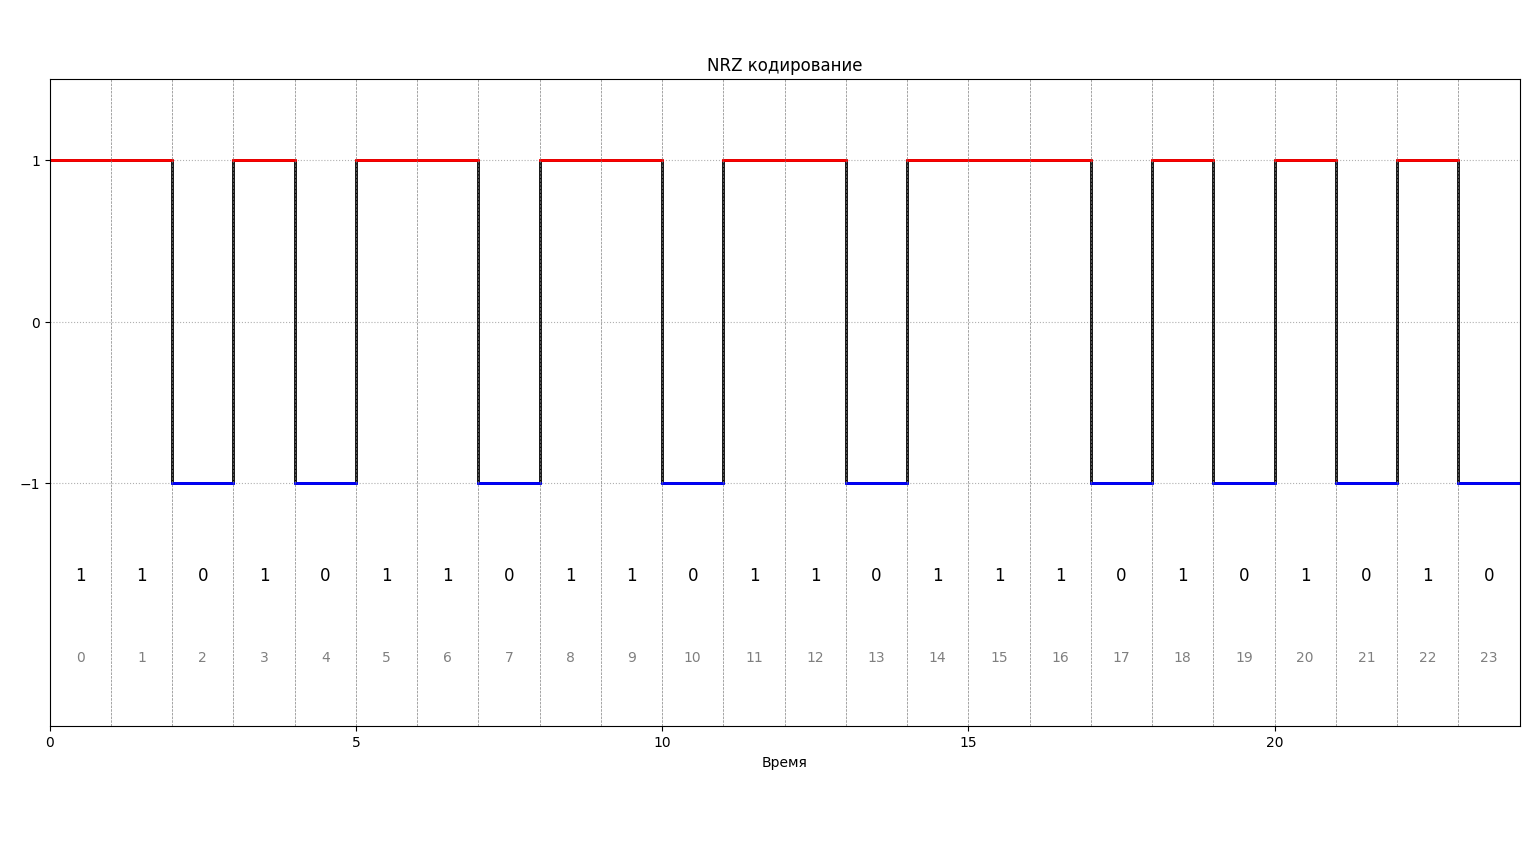
\includegraphics[width=\textwidth]{assets/nrz-scrambled.png}
\end{center}
\subsection*{Сравнительный анализ}
\begin{center}
    \begin{footnotesize}
        \hspace*{-2.9cm}
        \begin{tabular}{|c|c|c|c|c|c|c|}
            \hline
            \textbf{Метод} & \textbf{Пропускная с-ть} & \textbf{Спектр} & \textbf{Синхронизация} & \textbf{Обнаружение ошибок} & \textbf{Реализация} \\
            \hline
            4B/5B & Снижается & Сужается & Есть & Есть & Проще для человека \\
            \hline
            Скремблирование & Не меняется & Зависит & Нет & Нет & Проще для машины \\
            \hline
        \end{tabular}
    \end{footnotesize}
\end{center}
В результате сравнения анализов методов логического кодирования можно прийти к выводу что
избыточное кодирование имеет больше положительных критериев: спектр
всегда сужается, присутствуют синхронизация и обнаружение ошибок, но при этом падает пропускная способность.
При этом при использовании скремблирования пропускная способность сохраняется и такой вид кодирования
удобно реализовать с точки зрения компьютера

\subsection*{Вывод}
В ходе выполнения домашнего задания я познакомился с различными методами кодирования
сообщений: как физического, так и логического. Научился считать характеристики каждого из методов.
Проанализировал достоинства и недостатки каждого метода. Наглядно увидел то как работает каждый из методов и эффекты избыточного
кодирования
\end{document}
